\documentclass{ximera}

%\usepackage{todonotes}

\newcommand{\todo}{}

\usepackage{tkz-euclide}
\tikzset{>=stealth} %% cool arrow head
\tikzset{shorten <>/.style={ shorten >=#1, shorten <=#1 } } %% allows shorter vectors

\usepackage{tkz-tab}  %% sign charts
\usetikzlibrary{decorations.pathreplacing} 

\usetikzlibrary{backgrounds} %% for boxes around graphs
\usetikzlibrary{shapes,positioning}  %% Clouds and stars
\usetikzlibrary{matrix} %% for matrix
\usepgfplotslibrary{polar} %% for polar plots
\usetkzobj{all}
\usepackage[makeroom]{cancel} %% for strike outs
%\usepackage{mathtools} %% for pretty underbrace % Breaks Ximera
\usepackage{multicol}

\usepackage{polynom}



\usepackage[many]{tcolorbox}  %% for titled boxes
\newtcolorbox{xbox}[1]{%
    tikznode boxed title,
    enhanced,
    arc=0mm,
    interior style={white},
    attach boxed title to top center= {yshift=-\tcboxedtitleheight/2},
    fonttitle=\bfseries,
    colbacktitle=white,coltitle=black,
    boxed title style={size=normal,colframe=white,boxrule=0pt},
    title={#1}}


\usepackage{array}
\setlength{\extrarowheight}{+.1cm}   
\newdimen\digitwidth
\settowidth\digitwidth{9}
\def\divrule#1#2{
\noalign{\moveright#1\digitwidth
\vbox{\hrule width#2\digitwidth}}}





\newcommand{\RR}{\mathbb R}
\newcommand{\R}{\mathbb R}
\newcommand{\N}{\mathbb N}
\newcommand{\Z}{\mathbb Z}

%\renewcommand{\d}{\,d\!}
\renewcommand{\d}{\mathop{}\!d}
\newcommand{\dd}[2][]{\frac{\d #1}{\d #2}}
\newcommand{\pp}[2][]{\frac{\partial #1}{\partial #2}}
\renewcommand{\l}{\ell}
\newcommand{\ddx}{\frac{d}{\d x}}
\newcommand{\ddt}{\frac{d}{\d t}}

\newcommand{\zeroOverZero}{\ensuremath{\boldsymbol{\tfrac{0}{0}}}}
\newcommand{\inftyOverInfty}{\ensuremath{\boldsymbol{\tfrac{\infty}{\infty}}}}
\newcommand{\zeroOverInfty}{\ensuremath{\boldsymbol{\tfrac{0}{\infty}}}}
\newcommand{\zeroTimesInfty}{\ensuremath{\small\boldsymbol{0\cdot \infty}}}
\newcommand{\inftyMinusInfty}{\ensuremath{\small\boldsymbol{\infty - \infty}}}
\newcommand{\oneToInfty}{\ensuremath{\boldsymbol{1^\infty}}}
\newcommand{\zeroToZero}{\ensuremath{\boldsymbol{0^0}}}
\newcommand{\inftyToZero}{\ensuremath{\boldsymbol{\infty^0}}}



\newcommand{\numOverZero}{\ensuremath{\boldsymbol{\tfrac{\#}{0}}}}
\newcommand{\dfn}{\textbf}
%\newcommand{\unit}{\,\mathrm}
\newcommand{\unit}{\mathop{}\!\mathrm}
\newcommand{\eval}[1]{\bigg[ #1 \bigg]}
\newcommand{\seq}[1]{\left( #1 \right)}
\renewcommand{\epsilon}{\varepsilon}
\renewcommand{\iff}{\Leftrightarrow}

\DeclareMathOperator{\arccot}{arccot}
\DeclareMathOperator{\arcsec}{arcsec}
\DeclareMathOperator{\arccsc}{arccsc}
\DeclareMathOperator{\si}{Si}
\DeclareMathOperator{\proj}{proj}
\DeclareMathOperator{\scal}{scal}


\newcommand{\tightoverset}[2]{% for arrow vec
  \mathop{#2}\limits^{\vbox to -.5ex{\kern-0.75ex\hbox{$#1$}\vss}}}
\newcommand{\arrowvec}[1]{\tightoverset{\scriptstyle\rightharpoonup}{#1}}
\renewcommand{\vec}{\mathbf}
\newcommand{\veci}{\vec{i}}
\newcommand{\vecj}{\vec{j}}
\newcommand{\veck}{\vec{k}}
\newcommand{\vecl}{\boldsymbol{\l}}

\newcommand{\dotp}{\bullet}
\newcommand{\cross}{\boldsymbol\times}
\newcommand{\grad}{\boldsymbol\nabla}
\newcommand{\divergence}{\grad\dotp}
\newcommand{\curl}{\grad\cross}
%\DeclareMathOperator{\divergence}{divergence}
%\DeclareMathOperator{\curl}[1]{\grad\cross #1}


\colorlet{textColor}{black} 
\colorlet{background}{white}
\colorlet{penColor}{blue!50!black} % Color of a curve in a plot
\colorlet{penColor2}{red!50!black}% Color of a curve in a plot
\colorlet{penColor3}{red!50!blue} % Color of a curve in a plot
\colorlet{penColor4}{green!50!black} % Color of a curve in a plot
\colorlet{penColor5}{orange!80!black} % Color of a curve in a plot
\colorlet{fill1}{penColor!20} % Color of fill in a plot
\colorlet{fill2}{penColor2!20} % Color of fill in a plot
\colorlet{fillp}{fill1} % Color of positive area
\colorlet{filln}{penColor2!20} % Color of negative area
\colorlet{fill3}{penColor3!20} % Fill
\colorlet{fill4}{penColor4!20} % Fill
\colorlet{fill5}{penColor5!20} % Fill
\colorlet{gridColor}{gray!50} % Color of grid in a plot

\newcommand{\surfaceColor}{violet}
\newcommand{\surfaceColorTwo}{redyellow}
\newcommand{\sliceColor}{greenyellow}




\pgfmathdeclarefunction{gauss}{2}{% gives gaussian
  \pgfmathparse{1/(#2*sqrt(2*pi))*exp(-((x-#1)^2)/(2*#2^2))}%
}


%%%%%%%%%%%%%
%% Vectors
%%%%%%%%%%%%%

%% Simple horiz vectors
\renewcommand{\vector}[1]{\left\langle #1\right\rangle}


%% %% Complex Horiz Vectors with angle brackets
%% \makeatletter
%% \renewcommand{\vector}[2][ , ]{\left\langle%
%%   \def\nextitem{\def\nextitem{#1}}%
%%   \@for \el:=#2\do{\nextitem\el}\right\rangle%
%% }
%% \makeatother

%% %% Vertical Vectors
%% \def\vector#1{\begin{bmatrix}\vecListA#1,,\end{bmatrix}}
%% \def\vecListA#1,{\if,#1,\else #1\cr \expandafter \vecListA \fi}

%%%%%%%%%%%%%
%% End of vectors
%%%%%%%%%%%%%

%\newcommand{\fullwidth}{}
%\newcommand{\normalwidth}{}



%% makes a snazzy t-chart for evaluating functions
%\newenvironment{tchart}{\rowcolors{2}{}{background!90!textColor}\array}{\endarray}

%%This is to help with formatting on future title pages.
\newenvironment{sectionOutcomes}{}{} 



%% Flowchart stuff
%\tikzstyle{startstop} = [rectangle, rounded corners, minimum width=3cm, minimum height=1cm,text centered, draw=black]
%\tikzstyle{question} = [rectangle, minimum width=3cm, minimum height=1cm, text centered, draw=black]
%\tikzstyle{decision} = [trapezium, trapezium left angle=70, trapezium right angle=110, minimum width=3cm, minimum height=1cm, text centered, draw=black]
%\tikzstyle{question} = [rectangle, rounded corners, minimum width=3cm, minimum height=1cm,text centered, draw=black]
%\tikzstyle{process} = [rectangle, minimum width=3cm, minimum height=1cm, text centered, draw=black]
%\tikzstyle{decision} = [trapezium, trapezium left angle=70, trapezium right angle=110, minimum width=3cm, minimum height=1cm, text centered, draw=black]


\outcome{Solve basic related rates word problems.}
\outcome{Understand the process of solving related rates problems.}
\outcome{Calculate derivatives of expressions with multiple variables implicitly.}

\title[Dig-In:]{More than one rate}

\begin{document}
\begin{abstract}
  Here we work abstract related rates problems.
\end{abstract}
\maketitle


Suppose we have two variables $x$ and $y$ which are both changing with
respect to time.  A \textit{related rates} problem is a problem where
we know one rate at a given instant, and wish to find the other (the unknown rate is "related" to the known rate).

Here the chain rule is key: If $y$ is written in terms of $x$, and we
are given $\dd[x]{t}$, then it is easy to find $\dd[y]{t}$ using the
chain rule:
\[
y=y(x)
\]
\[
\dd[y]{t}=y'(x(t))\cdot x'(t).
\]
In many cases, particularly the interesting ones, our functions will
be related in some other way. Nevertheless, in each case we'll use the
power of the chain rule to help us find the desired rate. In this
section, we will work several abstract examples, so we can emphasize
the mathematical concepts involved. In each of the examples below, we
will follow essentially the same plan of attack:



\begin{description}
\item[\textbf{Introduce variables.}] Assign a variable to each quantity that changes in time.
\item[\textbf{Identify the given and unknown rates.}] 
\item[\textbf{Draw a picture.}] If possible, draw a schematic picture with all the relevant information. 
\item[\textbf{Find equations.}] Write equations that relate all
  relevant variables.
\item[\textbf{Differentiate with respect to time t.}] Here we will often use
  implicit differentiation and obtain an equation that relates the given rate and the unknown rate. 
\item[\textbf{Evaluate.}] Evaluate
each quantity at the  relevant moment.
 \item[\textbf{Solve.}] Solve
 for the unknown rate at that moment.
\end{description}




\section{Formulas}

One way to combine several variables is with a known formula.

\begin{example}
  Imagine an expanding circle. If we know that the perimeter is
  expanding at a rate of $4$ m/s, what rate is the area changing
  when the radius is $3$ meters?
  \begin{explanation}
   First, we \textbf{introduce the variables} $P$, $r$, and $A$. Let $P$ denote the perimeter of the circle, let $r$ denote the radius of the circle, and  let $A$ denote the area of the circle. Then, we \textbf{identify} the given rate $\frac{dP}{dt}=4$ m/s and the unknown rate $\Bigl[\frac{dA}{dt}\Bigr]_{r=3}$, the rate to be determined. 
    Next, we \textbf{draw a picture}.
    \begin{image}
      \begin{tikzpicture}
        \draw [penColor, very thick] (0,0) circle [radius=2];
        \draw [penColor] (0,0) -- (2,0);
        \node [below,penColor] at (1,0) {$r$ };
        \node [penColor,left] at (-1.5,1.42) {$\dfrac{d}{dt}P(t) = 4$ m/s};
        \node [penColor, right] at (1.5,-1.42) {$A = \pi\cdot r^2$};
      \end{tikzpicture}
    \end{image}
   Next, we \textbf{find equations} that combine relevant
   variables. Here we use the common formulas for perimeter and area
    \[
    P = \answer[given]{2\cdot \pi \cdot r}
    \qquad\text{and}\qquad
    A = \answer[given]{\pi \cdot r^2}.
    \]
   We know that the perimeter of the circle is expanding. This implies that both the radius and the area of the circle are changing in time, too.
    So, we note that $A$, $r$, and $P$ are functions of time
    \[
    P(t) = 2\cdot \pi \cdot r(t)
    \qquad\text{and}\qquad
    A(t) = \pi \cdot r(t)^2.
    \]
    We \textbf{differentiate} both sides of each equation using implicit
    differentiation, treating all functions as functions of $t$.
    \[
    \dfrac{d}{dt}P(t) = 2\cdot \pi\cdot  \dfrac{d}{dt}r(t)
    \qquad\text{and}\qquad
     \dfrac{d}{dt}A(t) = 2\cdot \pi\cdot r(t) \cdot  \dfrac{d}{dt}r(t).
    \]
    Now we \textbf{evaluate} all the quantities at the moment when $r=3$.
    
     We know  that at that moment $\Bigl[ \dfrac{d}{dt}P(t)\Bigr]_{r=3} =
    \answer[given]{4}$ and that $r = \answer[given]{3}$. Hence our
    equations become
    \[
    4 = 2\cdot \pi\cdot \Bigl[\dfrac{d}{dt}r(t)\Bigr]_{r=3}
    \qquad\text{and}\qquad
   \Bigl[ \dfrac{d}{dt}A(t)\Bigr]_{r=3} = 2\cdot \pi\cdot 3 \cdot \Bigl[\dfrac{d}{dt}r(t)  \Bigl]_{r=3}.
    \]
    We see that
    \begin{align*}
       4 &= 2\cdot \pi\cdot \Bigl[\dfrac{d}{dt}r(t)\Bigr]_{r=3}\\
      2/\pi &=  \Bigl[\dfrac{d}{dt}r(t)\Bigr]_{r=3}.
    \end{align*}
    Therefore, $\Bigl[\dfrac{d}{dt}r(t)\Bigr]_{r=3}= 2/\pi$ m/s.
   Now we \textbf{solve} for the rate of $A$ at the moment  when $r=3$.
   
    \begin{align*}
     \Bigl[ \dfrac{d}{dt}A(t)\Bigr]_{r=3} &= 2\cdot \pi\cdot 3 \cdot 2/\pi\\
      &=\answer[given]{12}.
    \end{align*}
    Hence the area is expanding at a rate of $12$ $m^2/s$ at the instant when $r=3$ m.
  \end{explanation}
\end{example}


%%BADBAD
%% There are a number of common formulas that arise in related rates
%% problems.
%%
%% It might be nice to add a little list of common area/volume formulas.



\section{Right triangles}

A common way to combine variables is through facts related to right
triangles.


\begin{example}
  Imagine an expanding right triangle. If one leg has a fixed length
  of $3$ m, one leg is increasing with a rate of $2$ m/s, and the
  hypotenuse is expanding to accommodate the expanding leg, at what
  rate is the hypotenuse expanding when both legs are $3$ m long?
  \begin{explanation}
 First, we \textbf{introduce the variables}  $a$, $b$, and $c$. Let $a$ denote the length of a leg with fixed length, let $b$ denote the length of a leg whose length is increasing, 
 and  let $c$ denote the length of the hypotenuse. Next, we \textbf{identify} the given rate $\frac{db}{dt}=2$ m/s and the unknown rate $\Bigl[\frac{dh}{dt}\Bigr]_{b=3}$, the rate to be determined.
   Now, we \textbf{draw a picture}.
    \begin{image}
      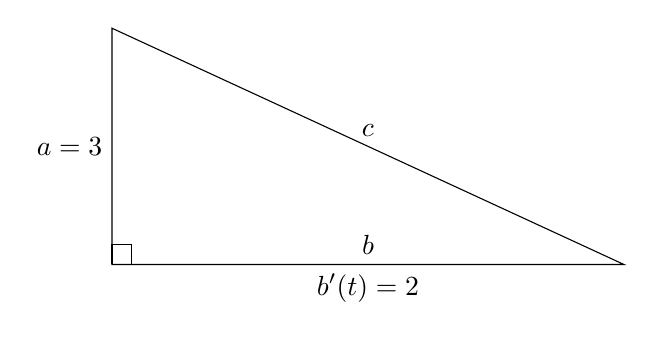
\begin{tikzpicture}
        \coordinate (A) at (0,2);
        \coordinate (B) at (0,5);
        \coordinate (C) at (6.5,2);
        \tkzMarkRightAngle(C,A,B)
        \tkzDefMidPoint(A,B) \tkzGetPoint{a}
        \tkzDefMidPoint(A,C) \tkzGetPoint{b}
        \tkzDefMidPoint(B,C) \tkzGetPoint{c}
        \draw (A)--(B)--(C)--cycle;
        \tkzLabelPoints[above](c)
        \tkzLabelPoints[above](b)
        %\tkzLabelPoints[left](a)
        \node [left] at (a) {$a = 3$};
        \node [below] at (b) {$b'(t) = 2$};
      \end{tikzpicture}
    \end{image}

    Next, we  \textbf{find equations} that combine relevant
    variables. Here we use the Pythagorean Theorem.
    \[
    c^2 = a^2 + b^2
    \]
   We note that $c$ and $b$ are functions of time, and write
    \[
    c(t)^2 = a^2 + b(t)^2.
    \]
    We \textbf{differentiate} both sides of the equation using
    implicit differentiation, treating all functions as functions of
    $t$, note $a$ is constant,
    \[
    2\cdot c(t)\cdot \dfrac{d}{dt}c(t) = 2\cdot b(t)\cdot \dfrac{d}{dt}b(t).
    \]
    Now, we \textbf{evaluate} all the quantities at the moment when $b=3$. We
    know that $\Bigl[\dfrac{d}{dt}b(t)\Bigr]_{b=3} = 2$ and that $b = 3$
    \[
    2\cdot [c(t)]_{b=3}\cdot \Bigl[\dfrac{d}{dt}c(t)\Bigr]_{b=3} = \answer[given]{12}
    \]
    However, we still need to know $[c(t)]_{b=3}$, the length of the hypotenuse at the moment when $b=3$. Here we use
    the Pythagorean Theorem,
    \begin{align*}
    \Bigl([c(t)]_{b=3}\Bigr)^2 &= 3^2 + 3^2\\
    &=\answer[given]{18},
    \end{align*}
    and so we see that $[c(t)]_{b=3} = 3\sqrt{2}$. \\
    And we \textbf{solve} for the rate.\\
    \begin{align*}
      6\sqrt{2}\cdot \Bigl[\dfrac{d}{dt}c(t)\Bigr]_{b=3} &= 12 \\     
      \Bigl[\dfrac{d}{dt}c(t)\Bigr]_{b=3} &= \sqrt{2}.
    \end{align*}
    Hence $c(t)$ is growing at a rate of $\answer[given]{\sqrt{2}}$ m/s when both legs are $3m$ long.
  \end{explanation}
\end{example}


\section{Angular rates}


We can also investigate problems involving angular rates.

\begin{example}
  Imagine an expanding right triangle. If one leg has a fixed length
  of $3$ m, one leg is increasing with a rate of $2$ m/s, and the
  hypotenuse is expanding to accommodate the expanding leg, at what
  rate is the angle opposite the fixed leg changing when both legs
  are $3$ m long?
  \begin{explanation}
  First, we \textbf{introduce the variables}  $a$, $b$, $c$, and $\theta$. Let $a$ denote the length of a leg with fixed length, let $b$ denote the length of a leg whose length is increasing, 
  let $c$ denote the length of the hypotenuse, and let $\theta$ denote the angle opposite the side with fixed length. Next, we \textbf{identify} the given rate $\frac{db}{dt}=2$ m/s and the unknown rate $\Bigl[\frac{d\theta}{dt}\Bigr]_{b=3}$, the rate to be determined.
    Next, we \textbf{draw a picture}.
    \begin{image}
      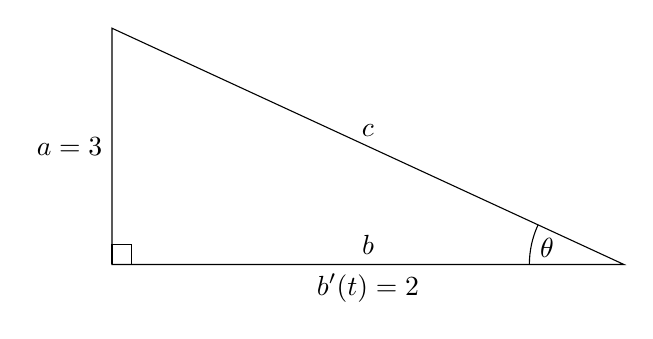
\begin{tikzpicture}
        \coordinate (A) at (0,2);
        \coordinate (B) at (0,5);
        \coordinate (C) at (6.5,2);
        \tkzMarkRightAngle(C,A,B)
        \tkzMarkAngle[size=1.2cm,thin](B,C,A)
        \tkzLabelAngle[pos = 1](B,C,A){$\theta$}
        \tkzDefMidPoint(A,B) \tkzGetPoint{a}
        \tkzDefMidPoint(A,C) \tkzGetPoint{b}
        \tkzDefMidPoint(B,C) \tkzGetPoint{c}
        \draw (A)--(B)--(C)--cycle;
        \tkzLabelPoints[above](c)
        \tkzLabelPoints[above](b)
        %\tkzLabelPoints[left](a)
        \node [left] at (a) {$a = 3$};
        \node [below] at (b) {$b'(t) = 2$};
      \end{tikzpicture}
    \end{image} 

    We now \textbf{find equations} that combine relevant
    functions. Here we note that
    \[
    \tan(\theta) = \answer[given]{\frac{a}{b}}
    \]
    Since $\theta$ and $b$ are functions of time, we write
    \[
    \tan(\theta(t)) = \frac{a}{b(t)}.
    \]
    We \textbf{differentiate}  both sides of  the equation using
    implicit differentiation, treating all functions as functions of
    $t$, note $a$ is constant,
    \[
    \sec^2(\theta(t))\theta'(t) = \frac{-a\cdot b'(t)}{b(t)^2}.
    \]
    Now we \textbf{evaluate} all the quantities at the moment when $b=3$.  We
    know that $a=3$, $b'(t) = 2$, and that $b = 3$
    \begin{align*}
    \Bigl[\sec^2(\theta(t))\Bigr]_{b=3}\cdot \Bigl[\dfrac{d}{dt}\theta(t)\Bigr]_{b=3} &= \frac{-3\cdot 2}{3^2}\\
    &= \frac{-6}{9}\\
    &= \frac{-2}{3}.
    \end{align*}
    However, we still need to compute $ \Bigl[\sec^2(\theta(t))\Bigr]_{b=3}$. Here we use the
    Pythagorean Theorem,
    \begin{align*}
    [c^2(t)]_{b=3} &= 3^2 + 3^2\\
    &=\answer[given]{18},
    \end{align*}
    and so we see that $[c(t)]_{b=3} = 3\sqrt{2}$. Now
    \begin{align*}
     \Bigl[\sec^2(\theta(t))\Bigr]_{b=3} &= \frac{\mathrm{hypotenuse}^2}{\mathrm{adjacent}^2}\\
      &= \frac{\left(3\sqrt{2}\right)^2}{3^2}\\
      &= \answer[given]{2}.
    \end{align*}
   Now we \textbf{solve}.
    \begin{align*}
    \Bigl[\sec^2(\theta(t))\Bigr]_{b=3}\cdot \Bigl[\dfrac{d}{dt}\theta(t)\Bigr]_{b=3}  &= \frac{-2}{3}\\
      2\cdot \Bigl[\dfrac{d}{dt}\theta(t)\Bigr]_{b=3}  &= \frac{-2}{3}\\
     \Bigl[\dfrac{d}{dt}\theta(t)\Bigr]_{b=3} &= \frac{-1}{3}.
    \end{align*}
    So when $a=b=3$, the angle is changing at $\answer[given]{-1/3}$
    radians per second.
  \end{explanation}
\end{example}



\section{Similar triangles}

Finally, facts about similar triangles are often useful when solving
related rates problems.

\begin{example}
  Imagine two right triangles that share an angle:
  \begin{image}
    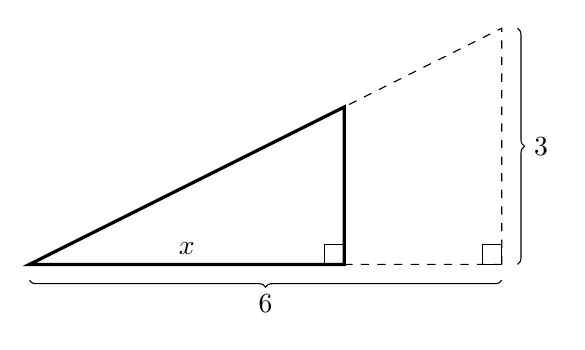
\begin{tikzpicture}
      \coordinate (A) at (6,2);
      \coordinate (B) at (6,5);
      \coordinate (C) at (0,2);
      \coordinate (D) at (4,2);
      \coordinate (E) at (4,4);
      \tkzMarkRightAngle(C,A,B)
      \tkzMarkRightAngle(C,D,E)
      \tkzDefMidPoint(A,B) \tkzGetPoint{a}
      \tkzDefMidPoint(A,C) \tkzGetPoint{b}
      \tkzDefMidPoint(D,C) \tkzGetPoint{x}
      \draw[decoration={brace,mirror,raise=.2cm},decorate,thin] (0,2)--(6,2);
      \draw[decoration={brace,mirror,raise=.2cm},decorate,thin] (6,2)--(6,5);
      \draw[dashed] (A)--(B)--(C)--cycle;
      \draw[very thick] (D)--(E)--(C)--cycle;
      \tkzLabelPoints[above](x)
      \node at (3,2-.5) {$6$};
      \node at (6+.5,3.5) {$3$};
    \end{tikzpicture}
  \end{image}
  If $x$ is growing from the vertex with a rate of $3$ m/s, what rate
  is the area of the smaller triangle changing when $x = 5$m?
  \begin{explanation}
  First, we \textbf{introduce the variables} $h$, the height of the smaller triangle, and $A$, the area of the smaller triangle.
Next, we \textbf{identify} the given rate $\frac{dx}{dt}=3$ m/s and the unknown rate $\Bigl[\frac{dA}{dt}\Bigr]_{x=5}$, the rate to be determined.
    Despite the fact that a nice picture is given, we should do what
    we always do and \textbf{draw a picture}. Note, we ad
    information to the picture:
    \begin{image}
      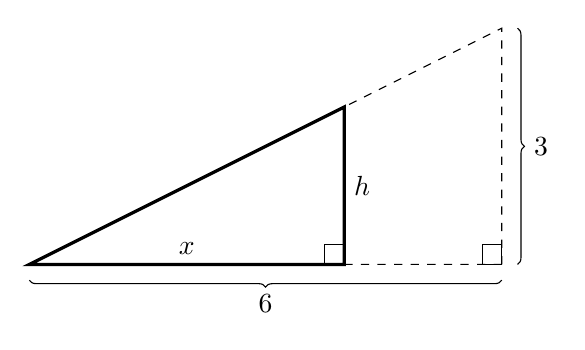
\begin{tikzpicture}
        \coordinate (A) at (6,2);
        \coordinate (B) at (6,5);
        \coordinate (C) at (0,2);
        \coordinate (D) at (4,2);
        \coordinate (E) at (4,4);
        \tkzMarkRightAngle(C,A,B)
        \tkzMarkRightAngle(C,D,E)
      \tkzDefMidPoint(A,B) \tkzGetPoint{a}
      \tkzDefMidPoint(A,C) \tkzGetPoint{b}
      \tkzDefMidPoint(D,C) \tkzGetPoint{x}
      \tkzDefMidPoint(D,E) \tkzGetPoint{h}
      \draw[decoration={brace,mirror,raise=.2cm},decorate,thin] (0,2)--(6,2);
      \draw[decoration={brace,mirror,raise=.2cm},decorate,thin] (6,2)--(6,5);
      \draw[dashed] (A)--(B)--(C)--cycle;
      \draw[very thick] (D)--(E)--(C)--cycle;
      \tkzLabelPoints[above](x)
      \tkzLabelPoints[right](h)
      \node at (3,2-.5) {$6$};
      \node at (6+.5,3.5) {$3$};
    \end{tikzpicture}
  \end{image}


    Next, we \textbf{find equations} that combine relevant
    variables. In this case there are two. The first is the formula
    for the area of a triangle:
    \[
    A = \answer[given]{(1/2) \cdot x \cdot h}
    \]
    The second uses the fact that the larger triangle is similar to
    the smaller triangle, meaning that the ratios between the corresponding sides in both triangles
    are equal,
    \[
    \frac{x}{h} = \answer[given]{\frac{6}{3}}\qquad\text{so}\qquad x =
    \answer[given]{2}\cdot h
    \]
   Since $A$, $x$, and $h$ are functions of time, we write
    \[
    A(t) = (1/2) \cdot x(t) \cdot h(t) \qquad\text{and}\qquad x(t) =
    2\cdot h(t).
    \]
    We now  \textbf{differentiate} both sides of each equation using
    implicit differentiation, treating all functions as functions of
    $t$,
    \begin{align*}
    \dfrac{d}{dt}A(t) &= (1/2) \cdot\dfrac{d}{dt}x(t) \cdot h(t) +  (1/2) \cdot x(t) \cdot \dfrac{d}{dt}h(t),\\
     \dfrac{d}{dt}x(t) &= 2\cdot\dfrac{d}{dt}h(t)
    \end{align*}
    Now we \textbf{evaluate} all the quantities at the moment when $x=5$m.
    \[
    5 = 2\cdot [h(t)]_{x=5}\qquad\text{and}\qquad 3= 2\cdot \Bigl[\dfrac{d}{dt}h(t)\Bigr]_{x=5}
    \]
    we see that $ [h(t)]_{x=5} = 5/2$ and $ \Bigl[\dfrac{d}{dt}h(t)\Bigr]_{x=5} = 3/2$. \\
    Now we \textbf{solve} for the rate.
    \begin{align*}
    \Bigl[\dfrac{d}{dt}A(t)\Bigr]_{x=5}  &= (1/2) \cdot 3 \cdot (5/2) + (1/2) \cdot 5 \cdot (3/2)\\
      &= 15/4 + 15/4\\
      &= \answer[given]{15/2}.
    \end{align*}
    Hence, the area is changing at a rate of $15/2$ $\text{m}^2/\text{s}$ when $x=5$m.
    
  \end{explanation}
\end{example}
\end{document}
